\begin{figure}[htb]
\centering
\includegraphics[page=6,width=0.33\textwidth]{\FCNCFigures/tthML/showFake/faketau/postfit/NOMINAL/reg1l2tau1bnj_ss/BDTG_test.pdf}
\put(-40, 90){\textbf{(a)}}
\put(-100, 90){\footnotesize{$t_l\thad\thad SS$}}
\includegraphics[page=6,width=0.33\textwidth]{\FCNCFigures/tthML/showFake/faketau/postfit/NOMINAL/reg1l2tau1bnj_ss/dphitauetmiss.pdf}
\put(-40, 90){\textbf{(b)}}
\put(-100, 90){\footnotesize{$t_l\thad\thad SS$}}
\includegraphics[page=6,width=0.33\textwidth]{\FCNCFigures/tthML/showFake/faketau/postfit/NOMINAL/reg1l2tau1bnj_ss/drlbditau.pdf}
\put(-40, 90){\textbf{(c)}}
\put(-120, 90){\footnotesize{$t_l\thad\thad SS$}}
\\
\includegraphics[page=6,width=0.33\textwidth]{\FCNCFigures/tthML/showFake/faketau/postfit/NOMINAL/reg1l2tau1bnj_ss/drlb.pdf}
\put(-40, 90){\textbf{(d)}}
\put(-128, 95){\footnotesize{$t_l\thad\thad SS$}}
\includegraphics[page=6,width=0.33\textwidth]{\FCNCFigures/tthML/showFake/faketau/postfit/NOMINAL/reg1l2tau1bnj_ss/drltau.pdf}
\put(-40, 90){\textbf{(e)}}
\put(-125, 90){\footnotesize{$t_l\thad\thad SS$}}
\includegraphics[page=6,width=0.33\textwidth]{\FCNCFigures/tthML/showFake/faketau/postfit/NOMINAL/reg1l2tau1bnj_ss/drtaub.pdf}
\put(-40, 90){\textbf{(f)}}
\put(-127, 95){\footnotesize{$t_l\thad\thad SS$}}
\\
\includegraphics[page=6,width=0.33\textwidth]{\FCNCFigures/tthML/showFake/faketau/postfit/NOMINAL/reg1l2tau1bnj_ss/drtaujmin.pdf}
\put(-40, 90){\textbf{(g)}}
\put(-100, 90){\footnotesize{$t_l\thad\thad SS$}}
\includegraphics[page=6,width=0.33\textwidth]{\FCNCFigures/tthML/showFake/faketau/postfit/NOMINAL/reg1l2tau1bnj_ss/drtautau.pdf}
\put(-40, 90){\textbf{(h)}}
\put(-60, 85){\footnotesize{$t_l\thad\thad SS$}}
\includegraphics[page=6,width=0.33\textwidth]{\FCNCFigures/tthML/showFake/faketau/postfit/NOMINAL/reg1l2tau1bnj_ss/etamax.pdf}
\put(-25, 100){\textbf{(i)}}
\put(-125, 95){\footnotesize{$t_l\thad\thad SS$}}
\\
\includegraphics[page=6,width=0.33\textwidth]{\FCNCFigures/tthML/showFake/faketau/postfit/NOMINAL/reg1l2tau1bnj_ss/etmiss.pdf}
\put(-40, 90){\textbf{(j)}}
\put(-100, 90){\footnotesize{$t_l\thad\thad SS$}}
\includegraphics[page=6,width=0.33\textwidth]{\FCNCFigures/tthML/showFake/faketau/postfit/NOMINAL/reg1l2tau1bnj_ss/lep_pt_0.pdf}
\put(-40, 90){\textbf{(k)}}
\put(-100, 90){\footnotesize{$t_l\thad\thad SS$}}
\includegraphics[page=6,width=0.33\textwidth]{\FCNCFigures/tthML/showFake/faketau/postfit/NOMINAL/reg1l2tau1bnj_ss/met_sigma.pdf}
\put(-40, 90){\textbf{(l)}}
\put(-100, 90){\footnotesize{$t_l\thad\thad SS$}}
\\
\caption{ Comparison of the variables distributions for the background and merged tuH signal in the $t_l\thadhad$ same sign control region. Only statistical uncertainties are being shown. Underflow and overflow bins are included respectively in the first and last bins.}
\label{fig:var_reg1l2tau1bnj_ss_1}
\end{figure}
\begin{figure}[htb]
\centering
\includegraphics[page=6,width=0.33\textwidth]{\FCNCFigures/tthML/showFake/faketau/postfit/NOMINAL/reg1l2tau1bnj_ss/mjjmin.pdf}
\put(-40, 90){\textbf{(a)}}
\put(-100, 90){\footnotesize{$t_l\thad\thad SS$}}
\includegraphics[page=6,width=0.33\textwidth]{\FCNCFigures/tthML/showFake/faketau/postfit/NOMINAL/reg1l2tau1bnj_ss/mtaujmin.pdf}
\put(-40, 90){\textbf{(b)}}
\put(-100, 90){\footnotesize{$t_l\thad\thad SS$}}
\includegraphics[page=6,width=0.33\textwidth]{\FCNCFigures/tthML/showFake/faketau/postfit/NOMINAL/reg1l2tau1bnj_ss/mtw.pdf}
\put(-40, 90){\textbf{(c)}}
\put(-65, 80){\footnotesize{$t_l\thad\thad SS$}}
\\
\includegraphics[page=6,width=0.33\textwidth]{\FCNCFigures/tthML/showFake/faketau/postfit/NOMINAL/reg1l2tau1bnj_ss/nljet.pdf}
\put(-40, 90){\textbf{(d)}}
\put(-100, 90){\footnotesize{$t_l\thad\thad SS$}}
\includegraphics[page=6,width=0.33\textwidth]{\FCNCFigures/tthML/showFake/faketau/postfit/NOMINAL/reg1l2tau1bnj_ss/phicent.pdf}
\put(-40, 90){\textbf{(e)}}
\put(-100, 90){\footnotesize{$t_l\thad\thad SS$}}
\includegraphics[page=6,width=0.33\textwidth]{\FCNCFigures/tthML/showFake/faketau/postfit/NOMINAL/reg1l2tau1bnj_ss/t1vismass.pdf}
\put(-40, 90){\textbf{(f)}}
\put(-120, 100){\footnotesize{$t_l\thad\thad SS$}}
\\
\includegraphics[page=6,width=0.33\textwidth]{\FCNCFigures/tthML/showFake/faketau/postfit/NOMINAL/reg1l2tau1bnj_ss/t2vismass.pdf}
\put(-40, 90){\textbf{(g)}}
\put(-100, 90){\footnotesize{$t_l\thad\thad SS$}}
\includegraphics[page=6,width=0.33\textwidth]{\FCNCFigures/tthML/showFake/faketau/postfit/NOMINAL/reg1l2tau1bnj_ss/tau_pt_0.pdf}
\put(-40, 90){\textbf{(h)}}
\put(-100, 90){\footnotesize{$t_l\thad\thad SS$}}
\includegraphics[page=6,width=0.33\textwidth]{\FCNCFigures/tthML/showFake/faketau/postfit/NOMINAL/reg1l2tau1bnj_ss/tau_pt_1.pdf}
\put(-40, 90){\textbf{(i)}}
\put(-100, 90){\footnotesize{$t_l\thad\thad SS$}}
\\
\includegraphics[page=6,width=0.33\textwidth]{\FCNCFigures/tthML/showFake/faketau/postfit/NOMINAL/reg1l2tau1bnj_ss/tautauvispt.pdf}
\put(-40, 90){\textbf{(j)}}
\put(-70, 70){\footnotesize{$t_l\thad\thad SS$}}
\includegraphics[page=6,width=0.33\textwidth]{\FCNCFigures/tthML/showFake/faketau/postfit/NOMINAL/reg1l2tau1bnj_ss/ttvismass.pdf}
\put(-40, 90){\textbf{(k)}}
\put(-70, 70){\footnotesize{$t_l\thad\thad SS$}}
\caption{Comparison of the variables distributions for the background and merged tuH signal in the $t_l\thadhad$ same sign control region. Only statistical uncertainties are being shown. Underflow and overflow bins are included respectively in the first and last bins.}
\label{fig:var_reg1l2tau1bnj_ss}
\end{figure}
